\documentclass[10pt, conference, letterpaper]{IEEEtran}
\usepackage{cite}
\usepackage{xcolor,soul,framed}
\usepackage{amsmath,amsthm,amssymb,amsfonts}
\usepackage{algorithmic}
\usepackage{graphicx}
\usepackage{color, soul}
\usepackage{algorithm, algorithmic}
\usepackage[utf8]{inputenc}
\usepackage[english]{babel}
\usepackage{mathtools}
\graphicspath{ {./images/} }

%---------------------------------------------------------------%
\newtheorem{definition}{Denifition}
\newtheorem{problem}{Problem}
\newtheorem{lemma}{Lemma}
\newtheorem{corollary}{Corollary}
\newtheorem{example}{Example}
\newcommand{\vecOne}{\mathbf{1}}
\newcommand{\ind}{\mathbf{I}}
\DeclarePairedDelimiter\set\{\}
%---------------------------------------------------------------%
\newcommand{\apSet}{\mathcal{K}}
\newcommand{\esSet}{\mathcal{M}}
\newcommand{\wSet}{\mathcal{W}}
\newcommand{\uSet}{\mathcal{U}}
\newcommand{\cSet}{\mathcal{C}}
\newcommand{\Stat}{\mathbf{S}}
%---------------------------------------------------------------%

\begin{document}

    %=============================== TITLE ===============================%
    \title{
        Meet-in-Future: Distributed Online Job Dispatching with Obsolete Information in Edge Computing System
    }
    \author{
        \IEEEauthorblockN{Yuncong Hong}
        \IEEEauthorblockA{
            \textit{Department of CS}, The University of Hong Kong, China \\
            ychong@cs.hku.hk
        }
    }
    \maketitle

    %============================== ABSTRACT ==============================%
    \begin{abstract}
        \label{sec:abstract}
        We formulate the problem with job dispatching in distributed Edge Computing system, and identify the difficulty exists in cooperation between APs (Access Points) and ESs (Edge Servers) with delayed information. In this work, we design the broadcast information in the system and formulate the corresponding problem into a MDP problem.
    \end{abstract}

    \begin{IEEEkeywords}
        Edge Computing, Job Dispatch, Delayed Information, Collective Observability, Distributed Multi-agent MDP
    \end{IEEEkeywords}

    %============================ INTRODUCTION ============================%
    \begin{section}{INTRODUCTION}
        \label{sec:introduction}
        (in progress)

        Some traits to mention compared to related works:
        \begin{itemize}
            \item we consider arrival process on ES may be affected by uploading process;
            \item we consider decentralized cooperation among APs without help from a centralized agent;
            \item we identify the delayed received broadcast information is un-acceptable, and it's hard to establish cooperation among APs because of obsolete information;
            \item we consider online job dispatching immediately without waiting for collective information and avoid the waiting time for decision.
        \end{itemize}
    \end{section}

    %========================= LITERATURE REVIEW ==========================%
    \begin{section}{LITERATURE REVIEW}
        \label{sec:review}
        Related work from \emph{Conference}:
        \begin{itemize}
            \item We use MDP definition in \cite{sutton1998introduction}
            \item The earliest related works we find is \cite{ref-01} (cited 167 times). In this work, the single agent is assumed not able to observe the global state, and thus they need communication to establish cooperation by sharing \emph{information}. The agent considers communication as extra action to synchronize the states and thus incurs extra cost. \\
            However, the communication is without delay, and converted into POMDP problem.
            \item The other work \cite{ref-02} considers continuous state observation with constant or stochastic delay with single agent. \\
            However, 
        \end{itemize}

        Realted work from \emph{Journal/Magazine}:
        \begin{itemize}
            \item (in progress...)
        \end{itemize}
    \end{section}

    %============================ SYSTEM MODEL ============================%
    \begin{section}{SYSTEM MODEL}
        \label{sec:model}
        mobile users (ME) offload jobs to access points (AP);
        APs makes decision to wait or upload to edge servers (ES);
        well-designed broadcast to help APs come to consensus on global states;
        In our problem, we consider \emph{response time} of jobs;

        \begin{subsection}{Network Model}
            We consider an MEC system topology illustrated in Fig. \ref{fig:system}.
            \begin{itemize}
                \item ME (Mobile Equipment) releases jobs to the corresponded AP (Access Point), and the MEs distribute within the coverage from all the APs considered in our system; (fully connected)
                \item AP has no computation power, and dispatches those jobs to ES (Edge Server);
                \item The uploading process is assumed parallel and with deterministic delay domained by propagation delay.
                \item The total uploading process could be divided into Fig. \ref{fig:trans} between the adjacent timeslots, using some \emph{indicator functions};
                \item for \emph{Parallel Uploading}: because the uploading time is finite and arrival frequency is at most 1 per timeslot, there actually needs finite channel capacity to serve the uploading process;
            \end{itemize}

            The communication model in our system ignores the underlaid physical property and association design.
            The assumed uploading time is deterministic and known in advance when the job is released to AP. The uploading time for one job may variance with respect to different ESs from the arrived AP, and the distribution of variance is not known in advance but is guaranteed with an expectation.
            Moreover, we assume the uploading process could be parallel among jobs which implies almost infinite capacity, and the end-to-end time is domain by the propagation time and processing time rather than communication time due to bandwidth. We identify this feature as the intrinsic property different from cloud computing scenario.
            \begin{figure}[ht]
                \centering
                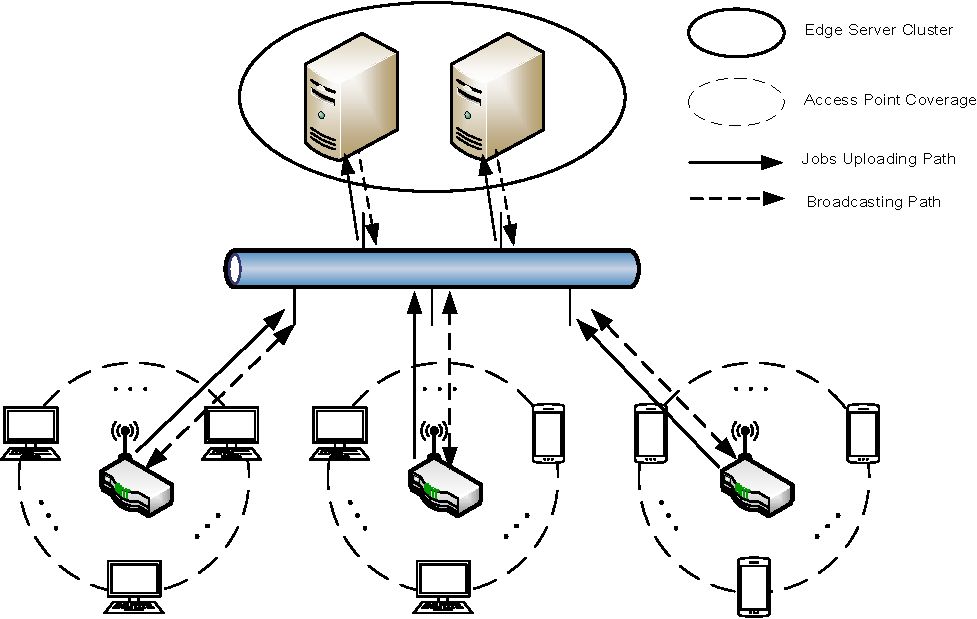
\includegraphics[width=0.45\textwidth, trim={0.5cm 0.5cm 0.5cm 0.5cm}, clip]{system-model.pdf}
                \caption{The Illustration of System Model}
                \label{fig:system}
            \end{figure}
                
            When the dispatching action is going to applied from AP agent's view, all the AP and ES nodes need to broadcast their local jobs' information for cooperation. The broadcast delay is considered deterministic and asynchronous at their own pace.
            The details of broadcast design about interval and contents will be elaborated in the following \textit{Broadcast Model} subsection.

            \begin{example}
                Task released; Action applied; Uploading; FCFS/SJF computation.
            \end{example}
        \end{subsection}

        \begin{subsection}{Computation Model}
            We assume that there is only one job being computed at one time on the edge server. The computation model is assumed to be deterministic.
            Moreover, we assume unrelated parallel machine model which implies that the computation time for one job is known when released but has no relationship among the edge servers.
        \end{subsection}

        \begin{subsection}{Broadcast Model}
            \begin{itemize}
                \item global aligned broadcast, and interval is far larger than the maximum delay from one nodes to the other AP nodes, i.e. $T \gg d$;
                \item consensus delay for $k$-th AP:
                    \begin{align}
                        \hat{d}_k = \max_{i\in(\mathcal{K} \cup \mathcal{N})}(d_{k,i})
                    \end{align}
            \end{itemize}

            The illustration figure \ref{fig:brd} for single broadcast includes several important time points which are also important in multiple synchronous broadcast: $x_{k,j}, d_{k,j}, T^{br}_{k,j}$
            \begin{figure}[ht]
                \centering
                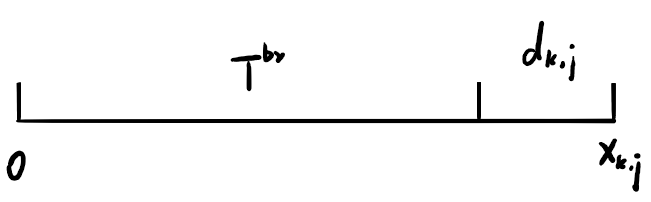
\includegraphics[width=0.45\textwidth]{single-broadcast.png}
                \caption{Single broadcast timing illustration}
                \label{fig:brd}
            \end{figure}
            And with the implication from the single broadcast, we generalize the conclusion for every broadcasts with:
            \begin{align}
                x_{k,j} = d_{k,j} + T^{br}_{j}
            \end{align}
            which takes a reasonable assumption that $T>d$ always ($j=k',n$ for $k$-th AP).
        \end{subsection}
    \end{section}

    %============================ FORMULATION =============================%
    \begin{section}{FORMULATION}
        \label{sec:formulation}
        \begin{itemize}
            \item We adapt \emph{timeslot} to characterize the minimum time slice in edge computing system, where the job release behavior from users is considered time-invariant in each time slot. And we use \emph{Bernoulli process} to characterize the memory-less behavior and there could be at most one job arrives in one timeslot.
            
            \item Let $\mathcal{K} \triangleq \set{1,\dots,K}$ to denote the AP nodes, $\mathcal{M} \triangleq \set{1,\dots,M}$ to denote ES nodes;
            
            \item \emph{Waiting Job Set} on $k$-th AP node in $t$-th timeslot as: $\wSet_{k}(t)$, $\forall k \in \apSet$;
            
            \item \emph{Uploading Job Set} from $k$-th AP to $m$-th ES in $t$-th timeslot as:
        \end{itemize}

        In this section we will firstly give out our optimization utility under a reasonable definition of edge computing system. As we are also considering cooperation among AP agents via a delicate broadcast design, we furthermore express the control policy decentralized on each AP agent.
        By leveraging a delicate broadcast design, all the AP agents could receive the local features about jobs at the broadcast point and the experienced local cost (number of jobs) during the broadcast interval.
        We formulate the local MDP optimization processes with the same target as the global optimization utility, but all with delayed cost to collect and delayed actions to apply based on the obsolete observation via broadcast. However, due to the different broadcast delay for each agents, the agents come to the consensus global states at different timeslot and thus compose the states transition, which is different from the situation with updated global information on each agents. We will discuss the difference and optimality gap at the end of this section.

        \begin{subsection}{Optimization Problem}
            We assume that there are $K$ APs and $N$ ESs in the MEC system.
            The arrival process of jobs at $k$-th AP is: $A^{(k)}(t)=I[t; L_C]$ which is a indicator random process. It will return $0$ if no jobs arrive at $t$-th time slot, and return the job with property $L_C$ if one job arrives, where $L_C$ is a vector of length $N$ denoting the deterministic computation time on unrelated machines.
            The computation time $L_C$ is bounded by $T_C$, i.e. $L_C \in [1,T_C]$.
                
            For one job $j$, it will wait until the uploading decision is made for it. Then it takes a general $T^{prop}_{k,n}$ time to be uploaded to $n$-th server from $k$-th access point; after being uploaded to $n$-th server, it will wait for its turn for computing until all the $L_C(n)$ components are processed and leave the system.

            \begin{definition}
                (Scheduling Policy). 
            \end{definition}
                
            Our optimization target is to minimize the average waiting time and computation time for each job, which is called the jobs' average response time. According to \emph{Little’s Law}, to minimize average response time, is equal to minimize the average number of jobs in a system, which is:
            \begin{problem}
                (Distributed Cooperative Job Dispatching)
                \begin{gather}
                    \min_{\Omega} \lim_{T \to \infty} E[\frac{1}{T} \sum_{t=0}^{T} N(t)]
                    \nonumber\\
                    N(t) = \sum_{k \in K} (A^{(k)}(t) + N_k(t))
                            + \sum_{n \in N} N_n(t)
                \end{gather}
            \end{problem}
            where $N_k(t)$ denotes the number of jobs on $k$-th AP, and $N_n(t)$ denotes the number of jobs on $n$-th ES.
            The goal to minimize the cost caused by ESs could be simply achieved with heuristic algorithm \emph{SJF} (shortest-job first), because it is the fastest way to reduce number of jobs on the edge server. So, in the next MDP problems we will focus on the policy applied on AP side, and leave ES with fixed heuristic algorithm.
        \end{subsection}

        \begin{subsection}{Standard MDP Formulation}
            We formulate the standard MDP problem in this section.

            \begin{subsubsection}{State and Cost}
                \begin{align}
                    T_t \triangleq \begin{pmatrix}
                        S_t \\ S_{t-1} \\ C_t
                    \end{pmatrix}, t=1,2,\dots
                \end{align}

                The transition for $(S_{t}, S_{t-1})$ is with policy $\vec{\Omega}(\tilde{S}_i)$ elaborated in the last section.
                
                While $C_t$ denotes the cost collected in the last broadcast interval, we have the expression as:
                \begin{align}
                    C_t = \sum_{t'\in[1,T^{br}]} \sum_{s'} P_{S_{t-1},s'}^{t'}(\vec{\beta}_{\Delta{t}}) \times |s'|
                \end{align}
                where,
                \begin{align}
                    P_{S_{t-1},s'}^{t'}(\vec{\beta}_{\Delta{t}})
                    = \{
                        \prod_{\Delta{t} \in [1,t']} P_{ss'}(\vec{\beta}_{\Delta{t}})
                    \}_{S_{t-1}, s'}
                \end{align}
            \end{subsubsection}

            \begin{subsubsection}{Action and Policy}
                Same as the definition in last section.
                \begin{align}
                    \vec{\Omega}(T_t) = \vec{\Omega}(\tilde{S}_t) \equiv \vec{\Omega}_{\Delta{t}}(S_t, S_{t-1})
                \end{align}
            \end{subsubsection}

            \begin{subsubsection}{Bellman Equation}
                \begin{align}
                    V(T_{t}) = C_t + \gamma \sum_{T_{t+1}} \Pr\{T_{t+1}|T_{t}, \vec{\Omega}(T_t)\} \cdot V(T_{t+1})
                \end{align}
            \end{subsubsection}
        \end{subsection}

        \begin{subsection}{Single-step Transition}
            We adapt the problem description at job-level grains and formulate the global states at $t$-th timeslot into job sets at APs and ESs:
            \begin{align}
                S(t) \triangleq
                \begin{Bmatrix}
                    S_{k}^{(W)}(t) = \{ (L_C) \}_{N_{k}^{(W)}}
                    \\
                    S_{k,n}^{(U)}(t)= \{ (L_C), L_{cd}^{(U)}(t) \}_{N_{k,n}^{(U)}}
                    \\
                    S_{n}^{(C)}(t)  = \{ L_{cd}^{(C)}(t) \}_{N_{n}^{(C)}}
                \end{Bmatrix}_{k\in\mathcal{K}, n\in\mathcal{N}}
            \end{align}
            where $L_C$ is a constant vector of length $N$ with each denoting the computation time of that job on each server; and $L^{(U)}_{cd}(t), L^{(C)}_{cd}(t)$ are countdowns for uploading and computing time remained for that job respectively.
            
            The single step transition graph is given below:
            \begin{figure}[ht]
                \centering
                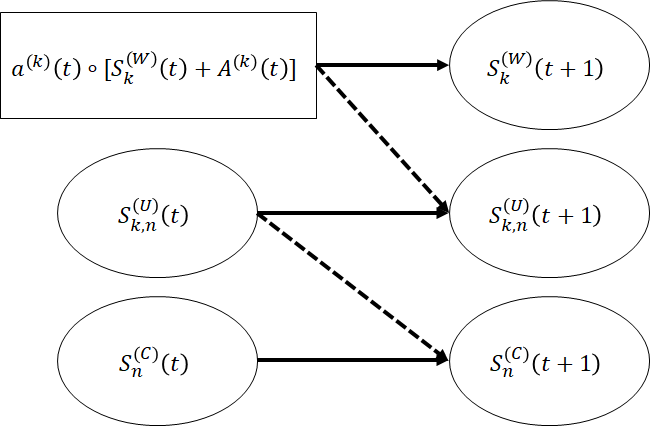
\includegraphics[width=0.45\textwidth]{single-transition.png}
                \caption{Single-step transition function composing graph}
                \label{fig:trans}
            \end{figure}
            Besides the states definition being illustrated above, we also have policy definition for $\vec{\Omega}(t) \triangleq (\Omega^{(1)}(t), \dots, \Omega^{(K)}(t))$ given the state $S(t)$. Each single policy $\Omega^{(k)}(t)$ defined on $k$-th AP is based on job-wise policy distribution $\vec{\alpha}^{(k)}$.

            The singleton action $a^{(k)}$ is defined for $k$-th AP as: for type-$j$ job, it should keep waiting or being uploaded to $n$-th server denoted as $\{0,1,\dots,N\}$. the action space is:
            \begin{align}
                A \triangleq \{a|a \in Z_*^{N+1}\}
            \end{align}
            As we have total $L_C^{N}$ kinds of jobs for all the unrelated machine, we have the set $\mathcal{J}=\{1, \dots, L_C^{N}\}$ denoting the job type index and the singleton policy on singleton action related with $j \in \mathcal{J}$ is:
            \begin{align}
                \vec{\alpha} \triangleq \{\alpha_1,\dots,\alpha_J\}
            \end{align}
            where $\alpha_j(a) \geq 0$ for all $a \in A$ and $\sum_a \alpha_j(a) = 1$.

            Then we give the denotations of a fixed job-wise policy distribution, which is called \emph{composed fixed policy} only related with $S^{(W)}(t), A^{(k)}(t)$ but not with the whole system features at $t$-th timeslot. The distribution for \emph{composed fixed policy} on $k$-th AP at $t$-th timeslot is given as:
            \begin{align}
                \Omega^{(k)}(t) &= \Pr\{a^{(k)}(j), \forall j \in S^{'(W)}_k(t) | A^{(k)}(t)\}
                \nonumber\\
                &= \prod_{j \in S^{'(W)}_k(t)} \alpha_{2^{(L_C)_j}}^{(k)}(a)
            \end{align}
            where $S^{'(W)}_k(t) \triangleq S^{(W)}_k(t) \cup A^{(k)}(t)$ and the decision on each job is based on the job type indexed with $2^{\vec{L_C}}$ and independent from each other. The output of this function gives the distribution of the \emph{joint uploading decision} of length $S^{'(W)}_k(t)$ on job set indexed with $\{1,\dots,|S^{'(W)}_k(t)|\}$.

            While the jobs processing is carried out following a descriptive procedure in the model section, we need some denotations to characterize the intrinsic of the transition. Firstly We come up with denotations for transition job sets expressed in figure \ref{fig:trans} as:
            \begin{align}
                I^{(W \to W')}_{k}(t) & \triangleq \{ j | a^{(k)}(j)=0, \forall j \in S^{'(W)}_k(t)\}
                \\
                I^{(W \to U)}_{k,n}(t) &\triangleq \{ j | a^{(k)}(j)=n, \forall j \in S^{'(W)}_k(t)\}
                \\
                I^{(U \to C)}_{k,n}(t) &\triangleq \{j|(L^{(U)}_{cd})_j=1, \forall j \in S^{(U)}_{k,n}(t)\}
                \\
                I^{(U \to U')}_{k,n}(t) &\triangleq S^{(U)}_{k,n}(t) \backslash I^{(U \to C)}_{k,n}(t)
                \\
                I^{(C \to \Phi)}_{n}(t) &\triangleq \{j|\arg\min_{j} (L^{(C)}_{cd})_j \wedge (L^{(C)}_{cd})_j=1\}
                \\
                I^{(C \to C')}_{n}(t) &\triangleq S^{(C)}_{n}(t) \backslash I^{(C \to \Phi)}_{n}(t)
            \end{align}
            Then we establish the relationship between those indicator functions with $S(t+1)$:
            \begin{align}
                \begin{cases}
                    S^{(W)}_{k}(t+1) = I^{(W \to W')}_{k}(t)
                    \\
                    S^{(U)}_{k,n}(t+1) = I^{(W \to U)}_{k,n}(t) + I^{(U \to U')}_{k,n}(t)
                    \\
                    S^{(C)}_{n}(t+1) = \sum_k I^{(U \to C)}_{k,n}(t) + I^{(C \to C')}_{n}(t)
                \end{cases}
            \end{align}
            And we note that only $I^{(W \to W')}_{k}(t)$ and $I^{(W \to U)}_{k,n}(t)$ are affected from disturbance from arrival process and randomized policy. With $\Omega^{(k)}(t)$ and $A^{(k)}(t)$ determined, we could obtain the joint distribution of local states on $k$-th AP as:
            \begin{align}
                & \Pr\{\begin{pmatrix}
                    S^{(W)}(t+1) \\ S^{(U)}(t+1)
                \end{pmatrix}
                |
                \begin{pmatrix}
                    S^{(W)}(t) \\ S^{(U)}(t)
                \end{pmatrix}, \vec{A}(t), \vec{\Omega}(t)
                \}
                \nonumber\\
                = &\prod_{k \in K} \Pr\{ A^{(k)}(t) \} \times \Omega^{(k)}(t)
            \end{align}

            On the server's side, the states transition is easily to obtain because the computation process on server is totally deterministic between adjacent timeslots:
            \begin{align}
                \Pr\{ S_{n}^{(C)}(t+1) |S_{n}^{(C)}(t), \{S_{k,n}^{(U)}(t)\}_{k \in \mathcal{K}} \} = 1
            \end{align}
            At last, we could come out with the global states transition function composed of the two parts as:
            \begin{align}
                & \Pr\{ S(t+1)|S(t), \vec{A}(t), \vec{\Omega}(t)  \}
                \nonumber\\
                = & \prod_{k \in K} \Pr\{ A^{(k)}(t) \} \times \Omega^{(k)}(t)
            \end{align}
        \end{subsection}

        \begin{subsection}{Multi-step Transition}
            We adapt aligned broadcast in practice where all of nodes will broadcast their local features at the point of broadcast and the cost collected in the broadcast interval.
            This joint information composes obsolete observations on all the AP nodes, and the nodes thus establish consensus on a global features. We assume that AP agents would take action on the one-step-backward obsolete observed states which result into a Markovian process and will be explained followed.

            We denote the collective global consensus observation on local features as:
            \begin{align*}
                & S_0, S_1, S_2, S_3, \dots
            \end{align*}
            where $S_i \triangleq S(iT^{br})$. it stresses that each agent all maintains the same $S_i$ for a $T^{br}$ period but not aligned due to different consensus delay $\hat{d}_k$ on each agent.

            In this consensus formulation illustrated in figure \ref{fig:br-trans}, we actually let every agents maintain the same global states with different deterministic delay. The delayed information doesn't impact on global states formulation of MDP problem, but converted into action over delayed states. For example, the agent would take actions based both on global states $S_1$ and $S_2$ in the period of $S_3$, because in the first half period it doesn't come to consensus on global states $S_2$.

            \begin{figure}[ht]
                \centering
                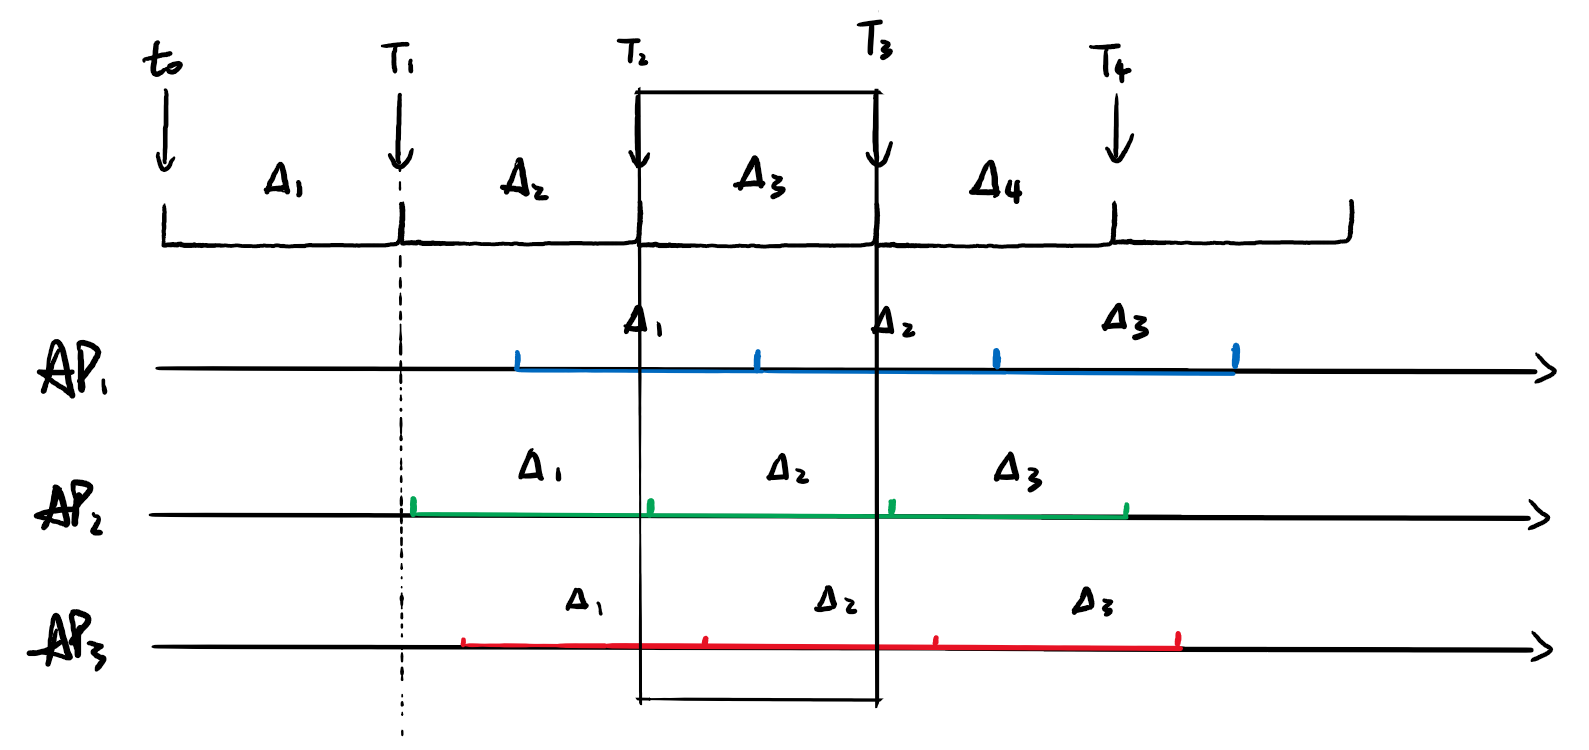
\includegraphics[width=0.45\textwidth]{broadcast-trans.png}
                \caption{Global Consensus and Transition with Delayed Action}
                \label{fig:br-trans}
            \end{figure}

            This implies that: \hl{The agents meet states in future with actions traced back into past}. The agents would contribute into global state transition, but the limited observation with obsolete information makes them always choose action based on the one-step-latter global states. So, one agent should carry out \emph{policy improvement} with other agents who fix their actions in its iteration. This improvement iteration comes to convergence always as the observations do not change with respect to policies.

            To formulate the transition between adjacent observation $S_i$ and $S_{i+1}$, we firstly give out the denotation for single-step transition with fixed action given previous state $s$ as:
            \begin{align}
                P_{ss'}(\vec{\beta}) \triangleq \Pr\{ S(t+1)=s'|S(t)=s, \vec{\Omega}(\vec{\beta},s|\vec{A}(t)),\vec{A}(t) \}
            \end{align}
            where $\vec{\beta} \triangleq (\vec{\alpha}^{(1)}, \dots, \vec{\alpha}^{(K)})$ is the fixed action vector on each nodes, and $\vec{\Omega}=\{\Omega^{(1)},\dots,\Omega^{(K)}\}$ with
            \begin{align}
                &\Omega^{(k)}(\vec{\alpha}^{(k)},s|A^{(k)}(t)) 
                = \prod_{j \in s \cup A^{(k)}(t)} \alpha_{2^{(L_C)_j}}^{(k)}(a)
            \end{align}
                
            Furthermore, we sort the index of APs with respect to their consensus delay $\hat{d}_k$ from small to big, i.e. $\hat{d}_1 \leq \hat{d}_2 \leq \dots \hat{d}_{K}$. This order is kept as a presumption in the follow parts. For the global broadcast interval $T^{br}$, the composed action denotations are given according to the consensus delays with $\Delta{t} \equiv t \pmod{T^{br}}$ as:
            \begin{align}
                &\vec{\Omega}_{\Delta{t}}(S_{i-1},S_{i}) = 
                \begin{cases}
                    \vec{\Omega}(\vec{\beta}(S_{i-1}, \dots, S_{i-1})) &,\; 0 \leq \Delta{t} < \hat{d}_1 \\
                    \vec{\Omega}(\vec{\beta}(S_{i}, S_{i-1}, \dots, S_{i-1})) &,\; \hat{d}_1 \leq \Delta{t}< \hat{d}_2 \\
                    \dots &,\; \dots \\
                    \vec{\Omega}(\vec{\beta}(S_{i}, S_{i}, \dots, S_{i})) &,\; \hat{d}_{K} \leq \Delta{t} < T^{br}
                \end{cases}
            \end{align}
            where,
            \begin{align}
                & \vec{\beta}(S_i,\dots, S_i,S_{i-1}, \dots,S_{i-1}) \triangleq \vec{\beta}_{\Delta{t}}
                \nonumber\\
                = & [\vec{\alpha}^{(1)}(S_i),\dots,\vec{\alpha}^{(k-1)}(S_i),
                    \vec{\alpha}^{(k)}(S_{i-1}),\dots,\vec{\alpha}^{(K)}(S_{i-1})]
            \end{align}
            and we have the one-step transition based on this composed policy definition as:
            \begin{align}
                P_{ss'}(\vec{\beta}_{\Delta{t}}) =& \prod_{k\in\mathcal{K}}{\Pr\{A^{(k)}(t)\}} \times \prod_{\hat{d}_k \leq \Delta{t}} { \Omega^{(k)}(\vec{\alpha}^{(k)}(S_{i}), s)}
                \nonumber \\
                & \times \prod_{\hat{d}_k > \Delta{t}} { \Omega^{(k)}(\vec{\alpha}^{(k)}(S_{i-1}), s) }
            \end{align}

            As the action defined on the latest observed states would actually latter two stages relative to next broadcast, we firstly establish the following transition function for the joint observation $\tilde{S}_i \triangleq (S_{i}, S_{i-1})$ as:
            \begin{align}
                & \Pr\{\tilde{S}_{i+1} | \tilde{S}_{i}, \vec{\Omega}(\tilde{S}_i)\}
                \nonumber\\
                = & \Pr\{S_{i+1}, S_{i} | S_{i},S_{i-1}, \vec{\Omega}(S_{i}), \vec{\Omega}(S_{i-1})\}
                \nonumber\\
                = & \{
                        \prod_{\Delta{t} \in [1,T^{br}]} P_{ss'}(\vec{\beta}_{\Delta{t}})
                    \}_{S_{i}, S_{i+1}}
            \end{align}
        \end{subsection}
        
    \end{section}

    %============================= ALGORITHM ==============================%
    \begin{section}{LOW-COMPLEXITY SOLUTION}
        \label{sec:algorithm}
        To alleviate the curse of dimensionality, we develope the approximate form of value function in the above illustrated problem. we adapt a heuristic baseline policy as the initial policy for the above illustrated problem.
        As the formulated problem above is of infinite states and the action space would be exponentially expanded with respect to number APs and ESs, we could not use traditional \emph{policy iteration} or \emph{value iteration} algorithm \cite{sutton1998introduction} for unacceptable computational complexity. To alleviate curse of dimensionality, we take one baseline policy to approximate the value function as $\tilde{V}(T_t)$ and carry out one-step iteration to come up with a better value function approximation.

        \begin{subsection}{Stochastic Process for Baseline Policy}
            \hl{Traditional value iteration is intractable due to the following reasons: (1) the number of active devices is not fixed and the state space grows exponentially with the increasing number of active devices; (2) the spaces of small-scale fading and path-loss are continuous.}

            The arrival process for jobs is assumed memory-less, i.e. invariant from time. According to \emph{Poisson Limit Theorem}, we adapt Bernoulli distribution for each timeslot with presence probability as $p_I$; the arrival distribution over the job set is:
            \begin{align*}
                \vec{p} = \{ p_0, p_1,\dots,p_J \}
            \end{align*}
            where $p_0=1-p_I$, and $p_0+\sum_{j=1}^{J}=1$.

            Firstly, we give the denotation of the jobs arrival distribution after a fixed action distribution $\alpha^{(k)}$ (not respect to states) for $k$-th AP as:
            \begin{align}
                \mathbf{I}^{(k)} &\triangleq \vec{\alpha}^{(k)} \circ A^{(k)}
                \nonumber\\
                &= \{ \vec{I}^{(k)}_{1}, \dots, \vec{I}^{(k)}_{J} \} = \{p^{(k)}_{j,n}\}
            \end{align}
            where, $p^{(k)}_{j,n} = p_j \times \alpha^{(k)}_j(a=n)$ for all $j \in \mathcal{J}$, $J=L_C^N$.
            The jobs after uploading decision would come to corresponding server after deterministic delay $T^{prop}_{k,n}$. However, we assume \emph{Bernoulli distribution} in each timeslot thus the arrival process $\mathbf{I}'^{(n)}$ for $n$-th server would actually be invariant from time.
            \begin{align}
                \mathbf{I}'^{(n)}(t) & = \{I'^{(n)}_1(t), \dots, I'^{(n)}_1(t) \}
                \\
                \vec{I}'^{(n)}_j(t) & = \sum_{k \in \mathcal{K}} p^{(k)}_{j,n}(t - T^{prop}_{k,n})
                \nonumber\\
                & = \vec{I}^{(k)}_{1} \times \vecOne
            \end{align}
            where $T^{prop}_{k,n}$ only matters in \emph{cost collection} from each AP node but not with arrival distribution. And the jobs of type $j$ would upload to $n$-th server with the corresponding component of length on that server. For convenience, we denote the mapping $f: (n,j) \to L_j(n)$ which obtains the mapping from probability distribution of \emph{jobs type} to \emph{jobs length on independent servers}, i.e. after being uploaded the length of job is determinant with $L_j(n)$.

            \begin{figure}[ht]
                \centering
                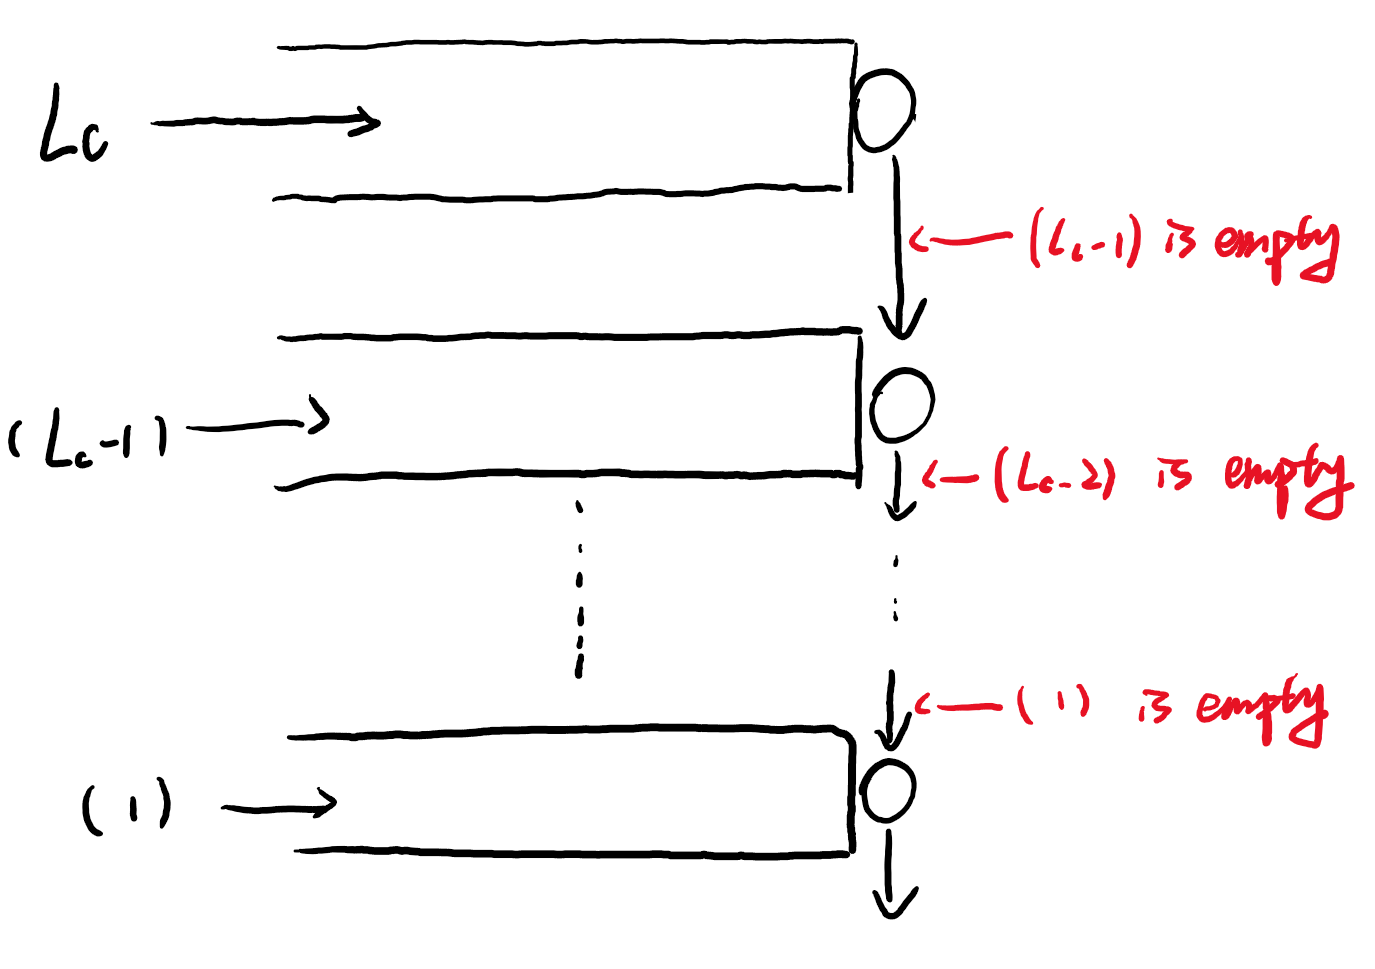
\includegraphics[width=0.45\textwidth]{srtf-graph.png}
                \caption{SRTF Job Transition between Multiple Queues}
                \label{fig:srtf}
            \end{figure}
            Then we give the denotation for structure of \emph{SRTF} process, which is illustrated in figure \ref{fig:srtf}. As \emph{SRTF} allows preemptive when new jobs arrive, we adapt multiple queues to record the number of different jobs of remaining time from $L_C$ to $1$. The spontaneous rule between the queues is: $j$-th queue will wait until all the $i$-th queues ($i < j$) are empty, then $j$-th queue could move one job to $(j-1)$-th queue in one timeslot and repeatedly moved until $1$-st queue then moved out.

            For given random variable $S^{(C)}_{n}(t)$, the denotation could be:
            \begin{align}
                S^{(C)}_{n}(t) \triangleq \begin{bmatrix}
                    X_{L_C} \\ \vdots \\X_{1}
                \end{bmatrix}
            \end{align}
            where $X_{l}$ changes following the deterministic \emph{SRTF} rule in adjacent timeslot. And according to the rule defined, we could obtain the turn-around time to remove all the jobs for $S^{(C)}_{n}(t)$ as:
            \begin{align}
                \begin{cases}
                    C(x_{1}) = \frac{x_1(x_1+1)}{2}
                    \\
                    C(x_{2}) = C(x_{1}) + 2 \cdot \frac{x_2(x_2+1)}{2}
                    \\
                    \dots
                    \\
                    C(x_{L_C}) = C(x_{1}) + \cdots + C(x_{L_C-1}) + L_C \cdot \frac{x_{L_C}(x_{L_C}+1)}{2}
                \end{cases}
            \end{align}
            and the sum-up turn-around time for all the jobs on $n$-th server at $t$-th timeslot is:
            \begin{align}
                C(S^{(c)}_{n}(t)) = \sum_{i=1}^{L_C} \frac{x_i(x_i+1)}{2} \cdot i(L_C-i+1)
            \end{align}
            The cost defined here is not instantaneous cost but the total cost brought by those current jobs.

            And we notice that the \emph{arrival injection} $I^{(n)}$, would only bring extra cost to current $C(S^{(c)}_{n}(t))$ with respect to independent components increase thus we don't have to simulate the \emph{preemption rule} for \emph{SRTF}. Thus the initial state $S^{(W)}(t), S^{(U)}(t)$ would \emph{finitely} affect the distribution on cost collection. However, the deterministic rule could be removed from cost collection by \emph{arrival injection}, but not from the state transition, which implies that we have to keep track of state transition with respect to the defined rule.

            At last, we collect the cost according to the definition in our MDP problem but with respect to our approximate algorithm.
            \begin{align}
                & \tilde{V}^{\pi}(T_t)
                \nonumber%\\
                = E_{\pi} \{ \tilde{C}_{t} + \gamma \tilde{C}_{t+1} + \gamma^2 \tilde{C}_{t+2} + \dots |S_{t-1}=s \}
                % \nonumber\\
                % = & \sum_{k=0}^{\infty} \gamma^{k} \sum_{t'=kT^{br}+1}^{(k+1)T^{br}} \sum_{s'} \tilde{P}^{t'}_{s,s'} \times |s'|
            \end{align}
            % where $\tilde{P}_{s,s'}$ is fixed under the given policy $\vec{\beta}_{\pi}$.
        \end{subsection}

        \begin{subsection}{The Distributed Algorithm}
            Then we introduce the one-step iteration algorithm in this section:
            % [\IF, \ENDIF], [\FOR, \TO, \ENDFOR], [\WHILE, \ENDWHILE], \STATE, \AND, \TRUE
            \begin{algorithm}[H]
                \caption{Distributed Algorithm for $k$-th AP}
                \begin{algorithmic}
                    \WHILE{\TRUE}
                        \STATE (in progress)
                        % \FOR{$k \in \mathcal{K}$}
                        %     \STATE fix policy $\vec{\Omega}^{(k)}(t) \forall k' \neq k$
                        % \ENDFOR
                    \ENDWHILE
                \end{algorithmic}
            \end{algorithm}
        \end{subsection}
        
    \end{section}

    %============================ EVALUATION ==============================%
    \begin{section}{EVALUATION}
        \label{sec:evaluation}
        (in progress)
    \end{section}

    %============================= CONCLUSION =============================%
    \begin{section}{CONCLUTION}
        \label{sec:conclusion}
        The future work to mention:
        \begin{itemize}
            \item non-aligned broadcast
            \item broadcast failure
            \item randomized broadcast delay
        \end{itemize}
    \end{section}

    %============================== REFERENCE =============================%
    \bibliographystyle{IEEEtran}
    \bibliography{main.bib}
\end{document}